\documentclass{article}
%%%%%%%%%%%%%%%%%%%%%%%%%%%%%%%%%%%%%%%
%% Makros & anderer Low-Level bastel %%
%%%%%%%%%%%%%%%%%%%%%%%%%%%%%%%%%%%%%%%
\makeatletter
%% Makros für Titel, Autor und Datum 
%% Dank diesem Makro stehen Titel, Autor und Datum überall im Dokument zur verfügung
%% Date hat zudem den Default-Wert \today
\def\@Title{}
\def\@Author{}
\def\@Date{\today}
\newcommand{\Title}{\@Title}
\newcommand{\Author}{\@Author}
\newcommand{\Date}{\@Date}
\AtBeginDocument{%
  \let\@Title\@title
  \let\@Author\@author
  \let\@Date\@date
}

%% Makros für den Arraystretch (bei uns meist in Tabellen genutzt, welche Formeln enthalten)
% Default Value
\def\@ArrayStretchDefault{1} % Entspricht der Voreinstellung von Latex

% Setzt einen neuen Wert für den arraystretch
\newcommand{\setArrayStretch}[1]{\renewcommand{\arraystretch}{#1}}

% Setzt den arraystretch zurück auf den default wert
\newcommand{\resetArrayStretch}{\renewcommand{\arraystretch}{\@ArrayStretchDefault}}

% Makro zum setzten des Default arraystretch. Kann nur in der Präambel verwendet werden.
\newcommand{\setDefaultArrayStretch}[1]{%
	\AtBeginDocument{%
		\def\@ArrayStretchDefault{#1}
		\renewcommand{\arraystretch}{#1}
	}
}
\makeatother


%%%%%%%%%%%%%%%%%%%%%%%
%% Wichtige Packages %%
%%%%%%%%%%%%%%%%%%%%%%%
\usepackage[utf8]{inputenc} % UTF-8 unterstützung
\usepackage[english, ngerman]{babel} % Silbentrennung
\usepackage[automark]{scrpage2} % Header und Footer
\usepackage{tabularx}

% Für Abbildungen mit mehreren kleinen Bilder
% Doku: http://www.ctan.org/tex-archive/macros/latex/contrib/caption/
\usepackage{caption}
\usepackage{subcaption}

\ifx \GUARDhsrColors \undefined
\def\GUARDhsrColors{}

\usepackage[table]{xcolor}

\definecolor{HSRWhite}{cmyk}{0,0,0,0}

\definecolor{HSRBlue}{cmyk}{1,0.4,0,0.2}
\definecolor{HSRBlue80}{cmyk}{0.8,0.32,0,0.16}
\definecolor{HSRBlue60}{cmyk}{0.6,0.24,0,0.12}
\definecolor{HSRBlue40}{cmyk}{0.4,0.16,0,0.08}
\definecolor{HSRBlue20}{cmyk}{0.2,0.08,0,0.04}

\definecolor{HSRLightGray}{cmyk}{0,0,0,0.30}
\definecolor{HSRLightGray80}{cmyk}{0,0,0,0.24}
\definecolor{HSRLightGray60}{cmyk}{0,0,0,0.18}
\definecolor{HSRLightGray40}{cmyk}{0,0,0,0.12}
\definecolor{HSRLightGray20}{cmyk}{0,0,0,0.06}

\definecolor{HSRSchwarz}{cmyk}{0,0,0,1}
\definecolor{HSRSchwarz80}{cmyk}{0,0,0,0.8}
\definecolor{HSRSchwarz60}{cmyk}{0,0,0,0.6}
\definecolor{HSRSchwarz40}{cmyk}{0,0,0,0.4}
\definecolor{HSRSchwarz20}{cmyk}{0,0,0,0.2}

\definecolor{HSRHematite}{cmyk}{0.6,1,0.4,0.2}
\definecolor{HSRHematite80}{cmyk}{0.48,0.80,0.32,0.16}
\definecolor{HSRHematite60}{cmyk}{0.36,0.60,0.24,0.12}
\definecolor{HSRHematite40}{cmyk}{0.24,0.40,0.16,0.08}
\definecolor{HSRHematite20}{cmyk}{0.12,0.20,0.08,0.04}

\definecolor{HSRLakeGreen}{cmyk}{0.70,0.30,0.45,0.05}
\definecolor{HSRLakeGreen80}{cmyk}{0.56,0.24,0.36,0.03}
\definecolor{HSRLakeGreen60}{cmyk}{0.42,0.18,0.27,0.02}
\definecolor{HSRLakeGreen40}{cmyk}{0.28,0.06,0.13,0.06}
\definecolor{HSRLakeGreen20}{cmyk}{0.14,0.06,0.09,0.01}

\definecolor{HSRReed}{cmyk}{0.10,0.25,0.45,0.60}
\definecolor{HSRReed80}{cmyk}{0.08,0.20,0.36,0.48}
\definecolor{HSRReed60}{cmyk}{0.06,0.15,0.27,0.36}
\definecolor{HSRReed40}{cmyk}{0.04,0.10,0.18,0.24}
\definecolor{HSRReed20}{cmyk}{0.02,0.05,0.09,0.12}

\definecolor{HSRPetrol}{cmyk}{1,0.18,0,0.45}
\definecolor{HSRPetrol80}{cmyk}{0.64,0.08,0.12,0.32}
\definecolor{HSRPetrol60}{cmyk}{0.48,0.06,0.09,0.24}
\definecolor{HSRPetrol40}{cmyk}{0.32,0.04,0.06,0.16}
\definecolor{HSRPetrol20}{cmyk}{0.16,0.02,0.03,0.08}

\definecolor{HSRBasswood}{cmyk}{0.25,0.05,0.70,0.15}
\definecolor{HSRBasswood80}{cmyk}{0.20,0.04,0.56,0.12}
\definecolor{HSRBasswood60}{cmyk}{0.15,0.03,0.42,0.09}
\definecolor{HSRBasswood40}{cmyk}{0.10,0.02,0.28,0.06}
\definecolor{HSRBasswood20}{cmyk}{0.05,0.01,0.14,0.03}


\fi
\ifx\GUARDmathe\undefined
\def\GUARDmathe{}

\usepackage{amssymb}
% Das mathtools package ist eine Erweiterung zum amsmath package.
% Das amsmath package wird dabei automatisch geladen
\usepackage{mathtools}


% Package mit vielen weiteren Mathe Symbolen
% http://www.ctan.org/tex-archive/fonts/mathabx
\usepackage{mathabx}

\fi
\ifx\GUARDenumitem\undefined
\def\GUARDenumitem{}

\usepackage{enumitem}

\fi

% Seitenränder für Formelsammlungen
\usepackage[left=1.9cm,right=1.9cm,top=1.9cm,bottom=1.9cm,includeheadfoot]{geometry}

\usepackage{multirow} % Create tabular cells spanning multiple rows
\usepackage{multicol} % In­ter­mix sin­gle and mul­ti­ple columns
\usepackage{rotating} % Rotation tools, including rotated fullpage floats


%%%%%%%%%%%%%%%%%%%%%%%%%%%%%%%%%%%
%% Layout der Kopf und Fusszeile %%
%%%%%%%%%%%%%%%%%%%%%%%%%%%%%%%%%%%
\deftripstyle{zusammenfassung}[0pt][0.5pt]
	{\Title}	% Kopfzeile innen
	{\headmark}	% Kopfzeile mitte
	{\pagemark}	% Kopfzeile aussen
	{\Author}	% Fusszeile innen
	{
\includegraphics[width=1.6cm]{./header/lizenzen/cc-by-nc-sa/small.png}}			% Fusszeile mitte
	{\Date}	% Fusszeile aussen
\pagestyle{zusammenfassung}



% Makros für Verweise auf ein Buch oder Skript
\newcommand{\buch}[1]{$_{\textcolor{HSRLakeGreen}{\mbox{\small{#1}}}}$}
\newcommand{\skript}[1]{$_{\textcolor{HSRReed}{\mbox{\small{#1}}}}$}

\setlength{\parindent}{0pt}
\ifx\GUARDhyperref\undefined
\def\GUARDhyperref{}

\ifx \GUARDhsrColors \undefined
\def\GUARDhsrColors{}

\usepackage[table]{xcolor}

\definecolor{HSRWhite}{cmyk}{0,0,0,0}

\definecolor{HSRBlue}{cmyk}{1,0.4,0,0.2}
\definecolor{HSRBlue80}{cmyk}{0.8,0.32,0,0.16}
\definecolor{HSRBlue60}{cmyk}{0.6,0.24,0,0.12}
\definecolor{HSRBlue40}{cmyk}{0.4,0.16,0,0.08}
\definecolor{HSRBlue20}{cmyk}{0.2,0.08,0,0.04}

\definecolor{HSRLightGray}{cmyk}{0,0,0,0.30}
\definecolor{HSRLightGray80}{cmyk}{0,0,0,0.24}
\definecolor{HSRLightGray60}{cmyk}{0,0,0,0.18}
\definecolor{HSRLightGray40}{cmyk}{0,0,0,0.12}
\definecolor{HSRLightGray20}{cmyk}{0,0,0,0.06}

\definecolor{HSRSchwarz}{cmyk}{0,0,0,1}
\definecolor{HSRSchwarz80}{cmyk}{0,0,0,0.8}
\definecolor{HSRSchwarz60}{cmyk}{0,0,0,0.6}
\definecolor{HSRSchwarz40}{cmyk}{0,0,0,0.4}
\definecolor{HSRSchwarz20}{cmyk}{0,0,0,0.2}

\definecolor{HSRHematite}{cmyk}{0.6,1,0.4,0.2}
\definecolor{HSRHematite80}{cmyk}{0.48,0.80,0.32,0.16}
\definecolor{HSRHematite60}{cmyk}{0.36,0.60,0.24,0.12}
\definecolor{HSRHematite40}{cmyk}{0.24,0.40,0.16,0.08}
\definecolor{HSRHematite20}{cmyk}{0.12,0.20,0.08,0.04}

\definecolor{HSRLakeGreen}{cmyk}{0.70,0.30,0.45,0.05}
\definecolor{HSRLakeGreen80}{cmyk}{0.56,0.24,0.36,0.03}
\definecolor{HSRLakeGreen60}{cmyk}{0.42,0.18,0.27,0.02}
\definecolor{HSRLakeGreen40}{cmyk}{0.28,0.06,0.13,0.06}
\definecolor{HSRLakeGreen20}{cmyk}{0.14,0.06,0.09,0.01}

\definecolor{HSRReed}{cmyk}{0.10,0.25,0.45,0.60}
\definecolor{HSRReed80}{cmyk}{0.08,0.20,0.36,0.48}
\definecolor{HSRReed60}{cmyk}{0.06,0.15,0.27,0.36}
\definecolor{HSRReed40}{cmyk}{0.04,0.10,0.18,0.24}
\definecolor{HSRReed20}{cmyk}{0.02,0.05,0.09,0.12}

\definecolor{HSRPetrol}{cmyk}{1,0.18,0,0.45}
\definecolor{HSRPetrol80}{cmyk}{0.64,0.08,0.12,0.32}
\definecolor{HSRPetrol60}{cmyk}{0.48,0.06,0.09,0.24}
\definecolor{HSRPetrol40}{cmyk}{0.32,0.04,0.06,0.16}
\definecolor{HSRPetrol20}{cmyk}{0.16,0.02,0.03,0.08}

\definecolor{HSRBasswood}{cmyk}{0.25,0.05,0.70,0.15}
\definecolor{HSRBasswood80}{cmyk}{0.20,0.04,0.56,0.12}
\definecolor{HSRBasswood60}{cmyk}{0.15,0.03,0.42,0.09}
\definecolor{HSRBasswood40}{cmyk}{0.10,0.02,0.28,0.06}
\definecolor{HSRBasswood20}{cmyk}{0.05,0.01,0.14,0.03}


\fi

\usepackage[plainpages=false,pdfpagelabels]{hyperref}
\hypersetup{
  pdfstartview={FitH}, % fits the width of the page to the window
  pdfauthor={\Author},
  pdfcreator={\Author},
  pdfproducer={\Author},
  pdftitle={\Title},
  colorlinks=true,
  linkcolor=HSRBlue,
  citecolor=HSRReed,
  filecolor=HSRLake,
  urlcolor=HSRHematite
}

\fi
\ifx\GUARDlistings\undefined
\def\GUARDlistings{}

\usepackage{listings}
\lstdefinestyle{Java}{ numbers=left,
  belowcaptionskip=1\baselineskip,
  breaklines=true,
  frame=L,
  xleftmargin=\parindent,
  language=Java,
  showstringspaces=false,
  basicstyle=\footnotesize\ttfamily,
  keywordstyle=\bfseries\color{green!40!black},
  commentstyle=\itshape\color{purple!40!black},
  identifierstyle=\color{blue},
  stringstyle=\color{orange},
  numberstyle=\ttfamily\tiny
}

\lstdefinestyle{SQL}{
  numbers=none,
  belowcaptionskip=1\baselineskip,
  breaklines=true,
  xleftmargin=\parindent,
  language=SQL,
  showstringspaces=false,
  basicstyle=\footnotesize\ttfamily,
  keywordstyle=\bfseries\color{green!40!black},
  commentstyle=\itshape\color{purple!40!black},
  identifierstyle=\color{blue},
  stringstyle=\color{orange},
}

\lstdefinestyle{C}{
  numbers=left,
  belowcaptionskip=1\baselineskip,
  breaklines=true,
  frame=L,
  xleftmargin=\parindent,
  language=C,
  showstringspaces=false,
  basicstyle=\footnotesize\ttfamily,
  keywordstyle=\bfseries\color{green!40!black},
  commentstyle=\itshape\color{purple!40!black},
  identifierstyle=\color{blue},
  stringstyle=\color{orange},
  numberstyle=\ttfamily\tiny
}

\lstdefinestyle{Cpp}{
  numbers=left,
  belowcaptionskip=1\baselineskip,
  breaklines=true,
  frame=L,
  xleftmargin=\parindent,
  language=C++,
  showstringspaces=false,
  basicstyle=\footnotesize\ttfamily,
  keywordstyle=\bfseries\color{green!40!black},
  commentstyle=\itshape\color{purple!40!black},
  identifierstyle=\color{blue},
  stringstyle=\color{orange},
  numberstyle=\ttfamily\tiny
}

\lstdefinestyle{Csharp}{
  numbers=left,
  belowcaptionskip=1\baselineskip,
  breaklines=true,
  frame=L,
  xleftmargin=\parindent,
  language=[Sharp]C,
  showstringspaces=false,
  basicstyle=\footnotesize\ttfamily,
  keywordstyle=\bfseries\color{green!40!black},
  commentstyle=\itshape\color{purple!40!black},
  identifierstyle=\color{blue},
  stringstyle=\color{orange},
  numberstyle=\ttfamily\tiny
}

\lstdefinestyle{Matlab}{
  numbers=left,
  belowcaptionskip=1\baselineskip,
  breaklines=true,
  frame=L,
  xleftmargin=\parindent,
  language=Matlab,
  showstringspaces=false,
  basicstyle=\footnotesize\ttfamily,
  keywordstyle=\bfseries\color{green!40!black},
  commentstyle=\itshape\color{purple!40!black},
  identifierstyle=\color{blue},
  stringstyle=\color{orange},
  numberstyle=\ttfamily\tiny
}

\fi

\setcounter{tocdepth}{2}
\setcounter{secnumdepth}{4} 
\numberwithin{equation}{section}
\numberwithin{figure}{section}

\usepackage{standalone}
\usepackage{cite}
\usepackage{tikz}
\usepackage{textcomp}
\usetikzlibrary{arrows,decorations.pathmorphing,positioning,fit,petri}
\usetikzlibrary{calc,intersections,through,backgrounds,graphs}
\usetikzlibrary{patterns,decorations.pathreplacing}

\title{Particle Swarm Optimization}
\author{Hannes Badertscher, Gregor Dengler}


%%%%%%%%%%%%
% Dokument %
%%%%%%%%%%%%
\begin{document}

	% Titelseite und Inhaltsverzeichnis
	% Title page and table of contents

\begin{titlepage}
	\vspace{2cm}
	\begin{center}
	{	\huge
		Particle Swarm Optimization
	}
	\end{center}
	
		
	\vspace{4cm}
	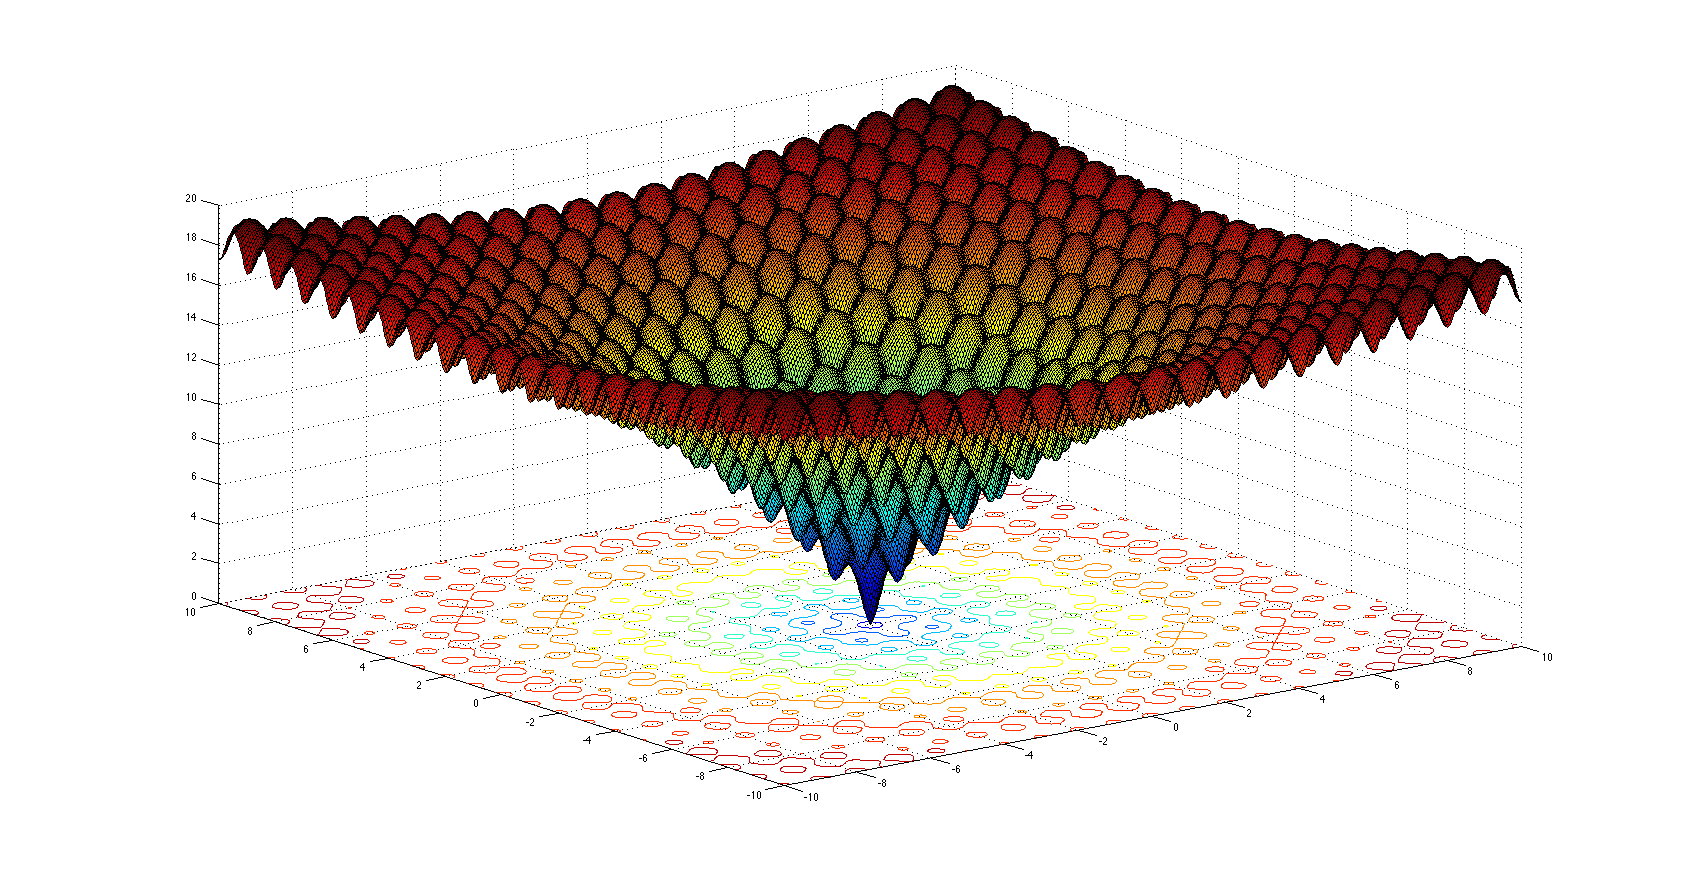
\includegraphics[height=10cm]{images/title.png}
	\vspace{4cm}
	
	\begin{center}
		\large
		Gregor Dengler, Hannes Badertscher \\
		\vspace{5mm}
		\Date
	\end{center}
	
	\thispagestyle{empty} % Don't start page numbers on this page
\end{titlepage}

\tableofcontents

\vspace{10mm}
{ \tiny
Title page: Ackley's Function
}
\newpage

	
	\section{Einführung}
		Die Partikelschwarmoptimierung wurde von James Kennedy \& Russel Eberhart im Jahre 1995 entwickelt. Es handelt sich um ein Nummerischen Optimierungsalgorithmus. Er simuliert das Verhalten von natürlichen Schwärmen um mathematische Problemstellungen zu optimieren.\\
		Es bewegt sich ein Schwarm von Partikel durch den Suchraum. Jedes Partikel hat eine Richtung und Geschwindigkeit sowie eine "Fitness". Die Fitness sagt aus wie gut die momentane Position ist. Partikel mit einer guten Fitness ziehen andere Partikel an, solche mit schlechter Fitness stossen andere Partikel ab. So beeinflussen sich die Partikel gegenseitig und man kann sehr viel Parallel berechnen, was vor allem bei Multicore Computersystemen von Vorteil ist. \\
		Diese Art von Optimierung wurde erst durch die Entwicklung von leistungsstarken Computersystemen möglich. Die ständig steigende Rechenleistung ermöglicht immer umfassendere Simulationen und damit immer umfassendere Optimierungen.
		\subsection{Schwarm}
		In der Natur gibt es viele verschiedene Strukturen und Formen in denen viele einzelne Bestandteile zusammen wirken. Eine davon ist ein Schwarm.\\
		Wenn man von Schwärmen spricht, denkt man an Fischschwärme oder an Vogelschwärme, die sich in der freien Wildbahn  bilden um z.B. als Zugvogelschwarm nach Süden oder Norden zu ziehen oder als Fischschwarm gemeinsam auf Nahrungssuche zu gehen oder sich gegen natürlich Feinde zu verteidigen. Solche Schwärme können das Wissen aller einzelnen Nutzen und so Beispielsweise die besten Futterplätze finden.
		\subsection{Schwarmintelligenz}
		Ein Schwarm kann als ganzes eine Eigenschaft haben, die aus den einzelnen Mitglieder des Schwarms nicht voraussagbar ist. So kann eine einzelne Nervenzelle keine Informationen Speicher oder denken. Wenn nun aber Milliarden von Nervenzellen richtig zusammen zu einem Hirn verknüpft sind, kann das ganze denke wie auch Informationen speichern. Dies sind offenbar emergente Eigenschaften, welche nicht durch einzelne Nervenzellen sonder durch ein vielzahl von Nervenzellen zustande kommt.
		\subsection{Emergenz}
		Emergente Eigenschaften sind Eigenschaften die durch das Zusammenspiel vom vielen einzelnen Teilen, zum Beispiel in einem Schwarm, entstehen. Diese Eigenschaften lassen sich nicht immer einzig aus den Bestandteilen des Schwarms vorhersagen. \\
		Das es ein Zusammenspiel von Bestandteilen ein Verhalten begründet, sagt noch nicht aus, dass dieses Verhalten automatisch Intelligenter ist, als das Verhalten der Bestanteilen selbst. In der Natur hat sich aber gezeigt, dass dieses emergente Verhalten oft wesentlich intelligenter ist, als das Verhalten von den einzelnen Bestandteilen. \\
		Die Emergenz ist Grundbestandteil von Algorithmen, welche auf das Verhalten von Schwärmen zurückgreifen.
		
		\subsection{Schwarmalgorithmus}

In den 1980er Jahren begann man das Verhalten von Schwärmen anhand von Computermodellen zu erforschen. Man wollte etwas über Evolution und deren Mechanismen lernen. Aus diesen Simulationen entstand der Schwarmalgorithmus.
In diesem Algorithmus wurden die Naturgesetze mit eingebaut, da man das Verhalten von Tieren in der freien Wildbahn erforschen wollte und diese auch diesen Naturgesetzen unterliegen.

\begin{itemize}
\item Vermeiden von Kollisionen 
\item Angleichen der Geschwindigkeit
\item Angleichen der Flugrichtung
\end{itemize}

Man stellte fest, dass es in solchen Schwärmen nicht möglich war, immer alle anderen Teilnehmer zu beachten, da die Schwärme sonst anfangen zu kreisen. Man fand heraus, das solche Schwärme in der Natur nicht zentral gesteuert werden, sondern es vielmehr ein Zusammenspiel vieler Teile ist, die sich gegenseitig beeinflussen.\\
Mit der Zeit entdeckte man, das solch ein Algorithmus auch zur Lösung von Optimierungsproblemen verwendet werden kann.
Man erkannte auch, dass beim Lösen von mathematischen Optimierungsproblemen die oben erwähnten Naturgesetze keine Rolle mehr spielen. Denn nun geht es nicht mehr um das Verhalten von Tierschwärmen in der freien Natur. Bei mathematischen Problemen ist es z.B. nicht so entscheidend, ob nun 2 Partikel zur selben Zeit am selben Ort sind (was in der Natur zu einer Kollision mit verletzten Tieren führt). So wurde der Schwarmalgorithmus zum Partikelschwarmalgorithmus entwickelt, welcher nicht zum Erforschen von Schwärmen in der Natur gedacht ist, sondern um Optimierungen zu berechnen.
				
		\subsubsection{Algorithmen}
		Es gibt verschiedene Alogrithmen, die die Schwarmintelligenz nutzen. Im Anschluss werden einige kurz vorgestellt. Am weitesten Verbreitet ist der Partikel Schwarmalgorithmus sowie der Ameisenalgorithmus, jedoch gibt es noch weiter Algorithmen, welche ebenfalls erforscht und weiterentwickelt werden. Auf diese Algorithmen wird im weitern nicht weiter eingegangen.
		
		\paragraph{Ant Colony Alogrithm}
		$\;$ \\
		Auch Ameisen nutzen die Intelligenz des Ganzen, wenn sie Futterplätze nutzen. Hat eine Ameise einen Futterplatz gefunden, hinterlässt sie auf dem Rückweg Pheromone, an denen sich andere Ameisen orientieren und so den Futterplatz und jeweils den Rückweg finden. Findet nun eine Ameise einen schnelleren Weg zurück so verflüchtigen sich diese Pheromone weniger schnell, da es weniger Zeit braucht für einen Weg. Nun werden die andere Ameisen aufmerksam auf diese stärkere Spur und schlussendlich nutzen alle diesen schnelleren Weg. Dieses Prinzip wird im Ameisenalgorithmus (ant colony optimization algorithm) ausgenützt.\\Dieser Algorithmus wird typischerweise für eine Pfadoptimierung verwendet.
		
		\paragraph{Invasive Weed}
		$\;$ \\
		Dieser Algorithmus orientiert an der Fortpflanzung von Pflanzen. Es werden Pflanzen frei über das Suchgebiet verteilt und dann die Fitness bewertet. Je Fitter eine Pflanze ist desto mehr Pflanzensamen verteilt sie. Auch bei diesen Pflanzen wird die Fitness bewertet. Das ganze wird solange fortgeführt, bis eine maximal Anzahl Pflanzen, die zuvor definiert wurde, erreicht ist und dann wird die Fitness aller Pflanzen bewertet und nur die der besten werden in einen neuen Durchgang mitgenommen. Dies wird solange wiederholt, bis das Abbruchkriterium erfüllt ist.
				
		
		\paragraph{Bees Algorithm}
		$\;$ \\
		Beim Bienenalgorithmus hat man, wie der Name schon sagt, bei den Bienen abgeschaut.\\
		In einem ersten Schritt werden \textacutedbl Scouts\textacutedbl \ frei über das Suchgebiet verteilt und im Anschluss deren Fitness angeschaut. Bei dem \textacutedbl Scout\textacutedbl \ mit der besten Fitness werden in der Umgebung erneut \textacutedbl Bienen\textacutedbl \ verteilt und deren Fitness beurteilt. Dieser Schritt wiederholt sich, bis man ein Ergebnis erreicht hat, das das Abbruchkriterium erfüllt.\\Dieser Algorithmus wird typischerweise für Kombinatorische oder funktionale Optimierung verwendet.
		
		\paragraph{Firefly Algorithm} 
		$\;$ \\
		Der Firefly Algorithm nutzt das Paarungsverhalten von Glühwürmchen. Glühwürmchen werden Unisexuel implementiert damit jedes Tier für das andere als Partner infrage kommt. \\
		Zuerst werden Glühwürmchen frei auf dem Suchgebiet verteilt. Danach wird die Fitness beurteilt. Je fitter ein Glühwürmchen ist, desto heller leuchtet es und je heller es leuchtet desto interessanter ist ein Glühwürmchen für die Artgenossen. Das heisst, jedes einzelne bewegt sich auf das Tier zu, das aus seiner Sicht am hellsten ist. Je näher man sich auf ein Glühwürmchen zu bewegt, desto heller leuchtet es. So werden bald alle Glühwürmchen Richtung Optimum wandern. Würden nun alle gleich hell leuchten, sprich dieselbe Fitness haben, würden sich die Tiere zufällig im Suchraum bewegen.
		
		
	\section{Partikelschwarm-Algorithmus}

\subsection{Algorithmus}
Für die Partikelschwarm-Optimierung sind folgende Zustandsdaten zu jedem Partikel notwendig:
\begin{align*}
	x_i: & \text{ aktuelle Position}\\
	v_i: & \text{ aktuelle Geschwindigkeit}\\
	p_i: & \text{ persönlich beste Position} \\
	l_i: & \text{ beste Position des Schwarms}
\end{align*} 

\subsubsection{Initialisierung}
Üblich ist die Initialisierung gemäss folgenden Formeln:
\begin{align}
	x_i(0) &= U(min,max) \\
	v_i(0) &= \frac{U(min,max) - x_i(0)}{2} \label{Vi-old} \\ 
	p_i(0) &= x_i(0)
\end{align}
Die Erfahrung hat gezeigt, dass mit der Initialisierung der Geschwindigkeit gemäss Gleichung \ref{Vi-old} die Partikel bei hohen Dimensionen den Suchraum praktisch unmittelbar verlassen. Um dies zu beheben wurde folgende angepasste Initialisierung eingeführt:
\begin{equation}
	v_i(0) = U(min - x_i(0), max - x_i(0))
\end{equation}

\subsubsection{Update der Geschwindigkeit}
Bei jeder Iteration werden die Zustandsdaten für jedes Partikel neu berechnet. Die neue Geschwindigkeit ist eine Linearkombination $\mathcal{C}$ von drei Vektoren: der aktuellen Geschwindigkeit, dem Abstand zur persönlich besten Position, sowie dem Abstand zur besten Position des Schwarms.
\begin{equation}
	v_{i}(t+1) = \mathcal{C}(v_i(t),\, p_i(t)-x_i(t),\, l_i(t)-x_i(t))
\end{equation}

Die Position wird nach der Geschwindigkeit gemäss Gleichung \ref{Pos-Update} aktualisiert. \\
\begin{equation}
	x_{i}(t+1) = x_i(t) + v_i(t+1) \label{Pos-Update}
\end{equation}

Über die korrekte Wahl der Linearkombination $\mathcal{C}$ wurden bereits ganze Arbeiten geschrieben. Weit verbreitet, wenn auch nicht ganz ideal ist die Berechnung gemäss Gleichung \ref{Vel-Update}. \\
\begin{equation}
	v_i(t+1) = w v_i(t) + U(0,c_1) (p_i(t)-x_i(t)) + U(0,c_2) (l_i(t)-x_i(t))\label{Vel-Update}
\end{equation}

mit den folgenden Parametern:
\begin{align*}
	w &: \text{Intertia Weight} \\
	c_1 &: \text{Cognitive Factor} \\
	c_2 &: \text{Social Factor}
\end{align*}
Diese Parameter, auch \textit{Acceleration Coefficients} genannt, beeinflussen das  Verhalten und die Konvergenz des Schwarms. Hohe $c_1$ und $c_2$ führen zu abrupteren Bewegungen und höheren Beschleunigungen. Mit der Gewichtung dieser beiden Faktoren lässt sich weiter einstellen, wie stark sich die Partikel von Schwarm beeinflussen lassen. Wie genau diese Parameter eingestellt werden ist von der Problemstellung abhängig. Gemäss Maurice Clerc \cite{Clerc-Stagnation} haben sich folgende Werte für die meisten Probleme als zweckmässig erwiesen:
\begin{equation}
	\left\lbrace \begin{array}{lllll}
		w & = & \frac{1}{2 \ln(2)} & \simeq & 0.721 \\
		c_1 = c_2 & = & \frac{1}{2} + \ln(2) & \simeq & 1.139 \\
	\end{array}	\right. 
\end{equation} \\


Die Herleitung der neuen Geschwindigkeit wird in Abbildung \ref{Fig-Visualisierung-Geschwindigkeit} visualisiert. Die Punkte $x'_i$ und $x''_i$ werden zufällig aus den zu den Achsen parallelen, gelb bzw. grün hinterlegten Bereichen generiert.  \\
\begin{figure}[htbp]
	\centering
	\documentclass{standalone}

\usepackage{tikz}
\usetikzlibrary{arrows,decorations.pathmorphing,positioning,fit,petri}
\usetikzlibrary{calc,intersections,through,backgrounds,graphs}
\usetikzlibrary{patterns,decorations.pathreplacing}

\begin{document}

\begin{tikzpicture}
	% Styles
	[
	point/.style={circle,draw=blue!50,fill=blue!20,thick, inner sep=0pt,minimum size=4mm},
	vpoint/.style={circle,draw=gray!50,fill=gray!20,thick, inner sep=0pt,minimum size=4mm},
	endpoint/.style={circle,draw=red!50,fill=red!20,thick, inner sep=0pt,minimum size=4mm},
	]
                      
	% Axis
	\draw[->] (0,0) -- (5,0);
  	\draw[->] (0,0) -- (0,5);
	
	% Shaded Parts
	\fill[gray!10!yellow!10] (1,1.5) rectangle (4.3,5.02);
	\fill[gray!10!green!10] (1,1.5) rectangle (4.85,0.4);

	% Nodes
	\node at (1.5,4.5)	(xi1)	[vpoint]	{};
	\node at (3,1.2)	(xi2)	[vpoint]	{};
	\node at (4,4.7)	(pi)	[point] 	{};
	\node at (4.5,0.5)	(li)	[point] 	{};
	\node at (1.7,-1)	(wvi) [point]	{};
	\node at (1,1.5)	(xi)	[point]	{} 
		edge [->,densely dotted]			(xi1)
		edge[densely dotted,gray]		(4.3,5.02)
		edge[->,densely dashdotted]		(xi2)
		edge[densely dashdotted,gray]	(4.85,0.4);
	\node at (4.2,1.7)	(xit)	[endpoint] {};
	\draw[->] (xi) -- (wvi);
	\draw[->,densely dotted] (wvi)  -- (2.2,2);
	\draw[->,densely dashdotted] (2.2,2) -- (xit);
	\draw[->,red!50]	(xi) -- (xit);

	% Text
	\node[blue!50]		at (0.6,1.5)	{$x_i$};
	\node[gray!50]		at (1.1,4.5) 	{$x'_i$};
	\node[gray!50]		at (3.5,1.2) 	{$x''_i$};
	\node[blue!50]		at (4,4.2)		{$p_i$};
	\node[blue!50]		at (4.2,0.2)	{$l_i$};
	\node[red!50]		at (4.2,2.2)	{$x_i(t+1)$};
	\node[blue!50]		at (1.1,-0.5)	{$wv_i$};

\end{tikzpicture}

\end{document}
	\caption{Visualisierung der Geschwindigkeit}
	\label{Fig-Visualisierung-Geschwindigkeit}
\end{figure}


\subsection{Grösse des Schwarms}
Über die ideale Grösse des Partikelschwarms lassen sich keine exakten Angaben machen. Gemäss \cite{Clerc-Standards} lässt sich die Grösse $S$ des Schwarms in Abhängigkeit der Dimension $D$ wie folgt ausdrücken:
\begin{equation}
	S = 10 + \left[ 2 \cdot \sqrt{D} \right]
\end{equation}
Die Näherung führt jedoch oft zu ungeeigneten Werten, weshalb Maurice Clerc vorschlägt, einen beliebigen Wert um $40$ zu wählen. Die theoretischen Grundlagen zur idealen Grösse des Schwarms sind nicht bekannt.


\subsection{Exploration-Exploitation Tradeoff}
Der Exploration-Exploitation Tradeoff sagt aus, dass ein Partikelschwarm nicht gleichzeitig ein möglichst grosses Zielgebiet absuchen kann (Exploration) und einen Bereich so genau wie möglich durchsuchen kann (Exploitation). Dieses Verhältnis von Exploration zu Exploitation hat einen starken Einfluss auf die Konvergenz. Generell kann gesagt werden, dass je höher die Inertia Weight $w$, desto weniger verlangsamt sich die Geschwindigkeit der Partikel, weshalb die Exploration stärker gewichtet wird.

\subsection{Parallelisierung}
Aus der Beschreibung des Algorithmus wird schnell ersichtlich, dass die Partikelschwarm-Optimierung sehr gut für eine parallelisierte Berechnung geeignet ist. Die Aktualisierung der Geschwindigkeit und Position kann für alle Partikel gleichzeitig, parallel erfolgen. Bei rechenintensiven Problemen ist dies ein enormer Vorteil gegenüber anderen Optimierungsmethoden.
	\section{Schwarm-Topologien}
Zum Bestimmen der sozialen Komponente des Geschwindigkeitsvektors kommen verschiedene Topologien oder Nachbarschaftsbeziehungen zur Anwendung. Diese Beziehungen unter den Partikeln haben einen essentiellen Einfluss auf den Algorithmus. Generell kann zwischen gbest (global best) und lbest (local best) unterschieden werden.

\begin{figure}[htbp]
	\centering
	\begin{minipage}{4cm}
		\centering
		\documentclass{standalone}

\usepackage{tikz}
\usetikzlibrary{arrows,decorations.pathmorphing,positioning,fit,petri}
\usetikzlibrary{calc,intersections,through,backgrounds,graphs}
\usetikzlibrary{patterns,decorations.pathreplacing}

\begin{document}

\begin{tikzpicture}
	% Styles
	[
	place/.style={circle,draw=blue!50,fill=blue!20,thick, inner sep=0pt,minimum size=4mm},
	]
                      
	% Nodes
	\node at (0,0.5)	(p1)	[place] {};
	\node at (0,1.5)	(p2)	[place] {};
	\node at (1,0)		(p3)	[place] {};
	\node at (1,2)		(p4)	[place] {};
	\node at (2,0.5)	(p5)	[place] {};
	\node at (2,1.5)	(p6)	[place] {};
	
	% Connections
	\graph[use existing nodes] {
		p1 -- p2; p1 -- p3; p1 -- p4; p1 -- p5; p1 -- p6;
		p2 -- p3; p2 -- p4; p2 -- p5; p2 -- p6;
		p3 -- p4; p3 -- p5; p3 -- p6;
		p4 -- p5; p4 -- p6;
		p5 -- p6;
	};
	

\end{tikzpicture}

\end{document}
		GBest
	\end{minipage}
	\begin{minipage}{4cm}
		\centering
		\documentclass{standalone}

\usepackage{tikz}
\usetikzlibrary{arrows,decorations.pathmorphing,positioning,fit,petri}
\usetikzlibrary{calc,intersections,through,backgrounds,graphs}
\usetikzlibrary{patterns,decorations.pathreplacing}

\begin{document}


\begin{tikzpicture}
	% Styles
	[
	place/.style={circle,draw=blue!50,fill=blue!20,thick, inner sep=0pt,minimum size=4mm},
	]
                      
	% Nodes
	\node at (0,0.5)	(p1)	[place] {};
	\node at (0,1.5)	(p2)	[place] {};
	\node at (1,0)		(p3)	[place] {};
	\node at (1,2)		(p4)	[place] {};
	\node at (2,0.5)	(p5)	[place] {};
	\node at (2,1.5)	(p6)	[place] {};
	
	% Connections
	\graph[use existing nodes] {
		p1 -- p2 -- p4 -- p6 -- p5 -- p3 -- p1;
	};
	

\end{tikzpicture}

\end{document}
		LBest - Ring
	\end{minipage}
	\begin{minipage}{4cm}
		\centering
		\documentclass{standalone}

\usepackage{tikz}
\usetikzlibrary{arrows,decorations.pathmorphing,positioning,fit,petri}
\usetikzlibrary{calc,intersections,through,backgrounds,graphs}
\usetikzlibrary{patterns,decorations.pathreplacing}

\begin{document}

\begin{tikzpicture}
	% Styles
	[
	place/.style={circle,draw=blue!50,fill=blue!20,thick, inner sep=0pt,minimum size=4mm},
	]
                      
	% Nodes
	\node at (0,0.5)	(p1)	[place] {};
	\node at (0,1.5)	(p2)	[place] {};
	\node at (1,0)		(p3)	[place] {};
	\node at (1,2)		(p4)	[place] {};
	\node at (2,0.5)	(p5)	[place] {};
	\node at (2,1.5)	(p6)	[place] {};
	
	% Connections
	\graph[use existing nodes] {
		p4 -- p1;
		p4 -- p2;
		p4 -- p3;
		p4 -- p5;
		p4 -- p6;
	};
	

\end{tikzpicture}

\end{document}
		LBest - Wheel
	\end{minipage}
	\begin{minipage}{4cm}
		\centering
		\documentclass{standalone}

\usepackage{tikz}
\usetikzlibrary{arrows,decorations.pathmorphing,positioning,fit,petri}
\usetikzlibrary{calc,intersections,through,backgrounds,graphs}
\usetikzlibrary{patterns,decorations.pathreplacing}

\begin{document}

\begin{tikzpicture}
	% Styles
	[
	place/.style={circle,draw=blue!50,fill=blue!20,thick, inner sep=0pt,minimum size=4mm},
	]
                      
	% Nodes
	\node at (0,0)	(p1)	[place] {};
	\node at (0,1)	(p2)	[place] {};
	\node at (0,2)	(p3)	[place] {};
	\node at (1,0)	(p4)	[place] {};
	\node at (1,1)	(p5)	[place] {};
	\node at (1,2)	(p6)	[place] {};
	\node at (2,0)	(p7)	[place] {};
	\node at (2,1)	(p8)	[place] {};
	\node at (2,2)	(p9)	[place] {};
	
	% Connections
	\graph[use existing nodes] {
		p1 -- p2 -- p3;
		p4 -- p5 -- p6;
		p7 -- p8 -- p9;
		p1 -- p4 -- p7;
		p2 -- p5 -- p8;
		p3 -- p6 -- p9;
	};

\end{tikzpicture}

\end{document}
		LBest - Von Neumann
	\end{minipage}
	\caption{Schwarm-Topologien}
\end{figure}

\subsection{GBest}
Die gbest Topologie geht von einem transparentem Partikelschwarm aus, in welchem die persönlich besten Positionen aller Partikel bekannt sind. Die soziale Komponente des gesamten Schwarms bildet sich also aus dem Abstand zur besten Position des gesamten Schwarms. Ein Vorteil dieser Nachbarschaftsbeziehung ist, dass der Schwarm schnell konvergiert, weil alle Partikel auf die momentan beste Position zulaufen.

\subsection{LBest}
Es existieren einige verschiedene lbest Architekturen. Die verbreitetsten lbest Architekturen sind oben dargestellt. Das Grundprinzip von lbest ist, dass jedes Partikel nur auf die besten Positionen seiner Nachbarn zugreifen kann. Wie die Nachbarpartikel bestimmt werden ist von der gewählten Topologie abhängig. Die lbest Methode hat den Vorteil, dass die Wahrscheinlichkeit gegen ein lokales Optimum zu konvergieren bedeutend kleiner ist. Dafür dauert es im Normalfall länger ein Optimum zu finden, als mit der gbest Methode.

\subsection{Wahl der Topologie}
Die Wahl der Topologie hängt stark von der Problemstellung ab. 

\subsection{Subpopulationen}
Um die Vorteile beider Topologien zu vereinen, kann das von genetischen Algorithmen (GA) bekannte Prinzip der Subpopulationen verwendet werden. Dabei wird der eigentliche Schwarm in mehrere Subpopulationen unterteilt, welche unabhängig von einander die PSO ausführen. Oft werden Subpopulationen verwendet, um einzelne Teilgebiete genauer untersuchen zu können.

\newpage

\subsubsection{HS-PSO}
Ein Spezialfall der Partikelschwarmoptimierung ist die hierarchical subpopulation PSO (HS-PSO), welche 2007 von Chuan Lin Quanyuan Feng (Southwest Jiaotong University) untersucht wurde. Das Prinzip der HS-PSO ist die Unterteilung des Schwarms nach einem hierarchischen Prinzip, wie in einer Unternehmung.

\begin{figure}[htbp]
	\centering
	\documentclass{standalone}

\usepackage{tikz}
\usetikzlibrary{arrows,decorations.pathmorphing,positioning,fit,petri}
\usetikzlibrary{calc,intersections,through,backgrounds,graphs}
\usetikzlibrary{patterns,decorations.pathreplacing}

\begin{document}

\begin{tikzpicture}
	% Styles
	[
	sub/.style={rectangle, rounded corners=3mm, minimum size=8mm, minimum width=1.2cm, draw=black!20, top color=white, bottom color=black!20},
	mid/.style={rectangle, rounded corners=3mm, minimum size=8mm, minimum width=1.5cm, draw=blue!20, top color=white, bottom color=blue!20},
	top/.style={rectangle, rounded corners=3mm, minimum size=8mm, minimum width=2cm, draw=red!20, top color=white, bottom color=red!20}
	]
                      
	% Nodes
	\node at (3.75,2.5)	(sub)	[top] {Sub};
	\node at (1.5,1.25)	(sub1)	[mid] {Sub1};
	\node at (6,1.25)	(sub2)	[mid] {Sub2};
	\node at (0,0)		(sub11)	[sub] {Sub11};
	\node at (1.5,0)	(sub12)	[sub] {Sub12};
	\node at (3,0)		(sub13)	[sub] {Sub13};
	\node at (4.5,0)	(sub21)	[sub] {Sub21};
	\node at (6,0)		(sub22)	[sub] {Sub22};
	\node at (7.5,0)	(sub23)	[sub] {Sub23};
	
	% Connections
	\graph[use existing nodes] {
		sub -- sub1;
		sub -- sub2;
		sub1 -- sub11;
		sub1 -- sub12;
		sub1 -- sub13;
		sub2 -- sub21;
		sub2 -- sub22;
		sub2 -- sub23;
	};

\end{tikzpicture}

\end{document}
	\caption{Hierarchical Subpopulation PSO}
\end{figure}

Die besten Partikel der Subpopulationen \textit{Sub11} - \textit{Sub13} bilden zusammen die Population \textit{Sub1}. Die besten Partikel der Populationen \textit{Sub1} - \textit{Sub2} bilden den Hauptschwarm \textit{Sub}. \\

Die einzelnen Partikelschwärme lassen sich unterschiedlich konfigurieren. So schlägt Chuan Lin vor, Schwärme in tiefen Hierarchiestufen auf das Erforschen des Gesamtgebiets einzustellen (d.h. geringe Sozialkomponente), während die höheren Hierarchiestufen relativ träge sind. Damit lässt sich ein grosses Gebiet erforschen, doch der Schwarm konvergiert kaum gegen lokale Minima. \\

In Benchmark-Tests haben HS-PSO Varianten bedeutend bessere Resultate als herkömmliche gbest und lbest Topologien hervorgebracht. Das Thema ist jedoch erst schwach erforscht. Weitere Arbeiten, vor allem zu adaptiven hierarchischen Strukturen und dem Informationsaustausch zwischen den Subpopulationen sind jedoch angekündigt.
	\section{Einschränkung des Zielgebiets}
Häufig kommt es vor, dass das Optimum innerhalb eines bestimmten Zielgebiets gesucht wird. Daher müssen Mittel gefunden werden die verhindern, dass die Partikel einen Definitionsbereich verlassen und nicht mehr zur Lösungsfindung beitragen. Die einfachste Möglichkeit ist, den Fitnesswert von Partikeln ausserhalb des Definitionsgebiets auf einen schlechten Wert zu setzen. Trotzdem benötigt das Partikel meist mehrere Iterationen um zurück in das Definitionsgebiet zu finden.

Eine verbreitete Lösung ist, das Partikel auf die Grenze des Bereichs und die Geschwindigkeit auf 0 zu setzen. Dieser Ansatz hat sich gegenüber dem ``Abprallen'' an der Bereichsgrenze durchgesetzt, weil so Optima am Rand des Zielgebiets besser erkannt werden können.

\section{Maximale Geschwindigkeit}
Ein bekanntes Problem der Partikelschwarm-Optimierung ist, dass die Geschwindigkeit eines Partikels schnell sehr hohe Werte annimmt. Das kann so weit gehen, dass ganze Teilgebiete durch die hohe Geschwindigkeit übersprungen werden. Die Lösung für dieses Problem ist die Einführung einer maximalen Geschwindigkeit, \textit{velocity clamping} genannt. Die Geschwindigkeit wird also nach folgender Formel berechnet:
\begin{equation}
	v_{ij}(t+1) = 
	\begin{cases}
		v_{ij}(t+1) & \text{if} |v_{ij}(t+1)| < V_{max,j} \\
		V_{max,j} & \text{if} |v_{ij}(t+1)| \geq V_{max,j}
	\end{cases}
	\label{eqn-max-velocity}
\end{equation}
Diese Erweiterung sorgt dafür, dass ein grösserer Bereich des Suchraums erforscht wird. Der optimale Wert für $V_{max,j}$ ist vom Problem abhängig und kann nicht generell bestimmt werden. \\

Wie die Gleichung \ref{eqn-max-velocity} zeigt, wird die Geschwindigkeit für jede Dimension einzeln beschränkt. Damit ergibt sich graphisch folgende Situation:

\begin{figure}[htbp]
	\centering
	\includegraphics{tikz/max-velocity.tex}
	\caption{Einführen einer maximalen Geschwindigkeit}
	\label{fig-max-velocity}
\end{figure}

Die Geschwindigkeit $v_2(t)$ ist hier grösser als die maximale Geschwindigkeit $V_{max}$, weshalb sie auf $v'_2$ reduziert wird. Die Geschwindigkeit $v_1$ wird jedoch nicht verändert. \\

Diese Geschwindigkeitsbegrenzung führt jedoch zu Problemen, wenn alle Geschwindigkeiten höher als die Begrenzung sind: Die Teilchen suchen dann nur an den Kanten eines $n$-dimensionalen Hyperwürfels. Als Gegenmassnahme kann gemäss \cite{schutte-sizing} $V_{max,j}$ dynamisch angepasst werden, wenn sich die global beste Position gbest über eine Anzahl $\tau$ Iterationen nicht verbessert:
\begin{equation}
	V_{max,j} = 
	\begin{cases}
		\beta V_{max,j} & \text{if} f(\hat{y}(t)) \geq f(\hat{y}(t-t')) 
			 \; \; \; \;  \forall \: t' = \{ 1, ..., \tau \} \\
		V_{max,j} & \text{otherwise}
	\end{cases}
\end{equation}
mit $0 < \beta < 1$ \\

Um eine höhere Genauigkeit zu erreichen kann die maximale Geschwindigkeit im Verlauf der Zeit exponentiell verringert werden:
\begin{equation}
	V_{max,j}(t+1) = \left(1-\left(\frac{t}{T}\right)^{\alpha}\right) V_{max,j}(t)
\end{equation}
$T$ ist hier die maximale Anzahl Iterationen. Der Faktor $\alpha$ ist abhängig von der Problemstellung und es existieren gemäss \cite{Han-Modification} keine mathematischen Hintergründe zur exakten Bestimmung. \\
	\section{Abbruchkriterien}

Da der Algorithmus theoretisch unendlich lange laufen kann, definiert man zu Beginn Abbruchkriterien, die den Algorithmus beenden.
Die Wahl der Abbruchkriterien kann einen bedeutenden Einfluss darauf haben, wie lange er läuft und ob er lokale oder globale Extremastellen findet.

\subsection{Art der Abbruchkriterien}

\subsubsection{Maximale Anzahl Iterationen}
Dies ist die einfachste Art, den Algorithmus zu beenden. Es bietet Vorteile, wie z.B. dass man von Anfang an weiss, wie lange der Algorithmus ungefähr laufen wird und dass es einfach zu Implementieren ist, da man sich keine Gedanken um den Wert des Ergebnisses machen muss. \\
Es gibt aber auch ein klaren Nachteil, man muss wissen wie lange der Algorithmus laufen muss, um das gewünschte Ziel zu erreichen. Es kann so passieren, dass man den Algorithmus abbricht, wenn er gerade bei einer lokalen Extremastelle ist oder sogar noch früher. Man hat bei diesem Abbruchkriterium keinen Einfluss auf die Qualität des Resultats, sondern nur auf die Zeit bis dieses gefunden wird.

\subsubsection{Schwellwert für den global besten Fitnesswert}
Mit diesem Abbruchkriterium legt man zu Beginn fest, welchen Fitnesswert man erreichen möchte und lässt den Algorithmus solange laufen, bis dieser erreicht ist.\\
Das Problem bei dieser Art von Abbruchkriterium ist, dass man keine Ahnung hat ob und wann der Algorithmus beendet wird. Es kann sein, das man einen Fitnesswert vorgibt, der gar nicht erst erreicht werden kann und der Algorithmus unendlich lange nach diesem Wert sucht. Sollte es kein Extrema geben läuft er ebenfalls unendlich lange. \textbf{Man muss also sicher stellen, das der Algorithmus noch ein weiteres Abbruchkriterium besitzt, da er sonst unendlich lange laufen kann.}

\subsubsection{Schwellwert für die minimale Veränderung der Funktionswerte}
Mit diesem Abbruchkriterium legt man fest, wie sehr sich die Funktionswerte bei jedem Durchgang verändern müssen. Ändern sich die Funktionswerte weniger als vorgegeben, wird der Algorithmus beendet. Es ist anzunehmen, das man sich sehr nahe an einem Extrema befindet und man unter Umständen bereits das gewünschte Resultat erreicht hat. Der Vorteil gegenüber dem Abbruchkriterium mit Schwellwert für den Fitnesswert ist, dass man hier nicht angeben muss, wie gut ein Ergebnis sein soll und somit kann auch ein Extrema gefunden werden, dass schlechter ist als erwartet. \\ 
Auch hier beseht die Gefahr, dass es sehr lange dauert bis der Algorithmus beendet wird. Man kann in der Regel nicht sagen, wie lang er laufen wird und sollte es kein globales Extrema geben, beseht die Gefahr, das er endlos läuft. 

\subsubsection{Schwellwert für den minimalen Bewegungsbereich}
In diesem Abbruchkriterium ist der minimale Bewegungsbereich vorgegeben. Bewegen sich die Partikel nur noch innerhalb des Bereichs, wird der Prozess beendet. Man kann davon ausgehen, das sich innerhalb des Bereichs auch das Extrema befindet und man einen genügend guten Fitnesswert erreicht hat. Mit diesem Kriterium kann analog zu oben ebenfalls ein Extrema gefunden werden, welches schlechter ist als erwartet.\\
Bei diesem Abbruchkriterium ist ebenfalls zu beachten, dass es nur abbricht, wenn ein Extrema vorhanden ist. Sollte es keines geben, läuft er endlos.

\subsection{Wahl der Abbruchkriterien}
Die Wahl der Abbruchkriterien ist sehr wichtig, wenn man mit der Partikelschwarmoptimierung etwas erreichen will. Man muss festlegen, ob die Zeit der Berechnung oder die Qualität des Resultats wichtiger sind. Ist die Zeit das Ausschlaggebende gibt man die maximale Anzahl Iterationen vor. Hat man genügend Zeit zum berechnen, gibt man nebst einer maximalen Anzahl Iterationen noch eines der anderen Kriterien vor und kann so mit der Anzahl Iterationen die maximale Zeit steuern und mit dem anderen Kriterium die Qualität. 


	\section{Anwendungen}
	\section{Code}
Der komplette C++ Code befindet sich im Anhang. In diesem Teil wird der Code beschrieben.

\subsection{Position-Klasse}
Die Klasse \textit{Position} stellt einen mehrdimensionalen Datentyp zur Verfügung. 
Damit ist es möglich, Probleme jeder beliebigen Dimension zu lösen.

\subsection{Particle-Klasse}
In der \textit{Particle}-Klasse werden die Positionen und Geschwindigkeiten jedes Partikels
als Attribute gespeichert. Weiter werden Funktionen für Geschwindigkeits- und Positionsupdates
zur Verfügung gestellt.

\subsection{Swarm-Klasse}
Die Klasse \textit{Swarm} dient dazu, einen Schwarm von Partikeln zu erzeugen und zu initialisieren.
Zusätzlich wird eine Funktion zur Ausführung der Optimierung bereitgestellt.

\subsection{Random}
Die selbst erstellte Funktion \textit{getRand} dient dazu, Zufallszahlen im Bereich zwischen \textit{min} und \textit{max} zu erzeugen. Diese werden in der Initialisierung und bei jeder Iteration des Schwarms benötigt. 
	
	\newpage
	\bibliographystyle{plain}
	\bibliography{literature}
	
	\newpage
	\section{Anhang}
	\subsection{Swarm.h / Swarm.cpp}
	\lstinputlisting[language=C++]{PSO-Code/Swarm.h}
	\lstinputlisting[language=C++]{PSO-Code/Swarm.cpp}
	\subsection{Particle.h / Particle.cpp}
	\lstinputlisting[language=C++]{PSO-Code/Particle.h}
	\lstinputlisting[language=C++]{PSO-Code/Particle.cpp}
	\subsection{Position.h / Position.cpp}
	\lstinputlisting[language=C++]{PSO-Code/Position.h}
	\lstinputlisting[language=C++]{PSO-Code/Position.cpp}
	\subsection{Random.h / Random.cpp}
	\lstinputlisting[language=C++]{PSO-Code/Random.h}
	\lstinputlisting[language=C++]{PSO-Code/Random.cpp}
	\subsection{main.cpp}
	\lstinputlisting[language=C++]{PSO-Code/main.cpp}
	
\end{document}